\documentclass[11pt]{article}
\usepackage[margin=1in]{geometry}
\usepackage{amsmath,amssymb}
\usepackage{listings}
\usepackage{xcolor}
\usepackage[colorlinks=true,linkcolor=blue,urlcolor=blue]{hyperref}
\usepackage{tikz}

\lstdefinestyle{lean}{
  basicstyle=\ttfamily\small,
  breaklines=true,
  backgroundcolor=\color{gray!8},
  frame=single,
  framesep=6pt,
  xleftmargin=4pt,
  keywordstyle=\color{purple!70!black}\bfseries,
  morekeywords={theorem,def,Prop,Set,Real,fun,MeasureTheory,volume,axioms},
  commentstyle=\color{green!40!black}\itshape,
  morecomment=[l]{--},
}

\title{A formally verified theorem:\\
the smallest ellipse holding two unit circles has area $\tfrac{3\sqrt3}{2}\pi$\\[4pt]
\large What the Lean statement says, and why it needed a proof}
\author{}
\date{}

\begin{document}
\maketitle

\section{The result in one sentence}

Among all ellipses that contain two unit-radius circles with disjoint interiors, the one of
\emph{smallest area} has area exactly
\[
  A \;=\; \frac{3\sqrt3}{2}\,\pi \;\approx\; 8.1621,
\]
achieved by the ellipse $\frac{x^2}{9/2}+\frac{y^2}{3/2}\le 1$ with the two unit circles centred at
$(\pm1,0)$, touching at the origin. Each circle is internally tangent to the ellipse at two points.

\begin{center}
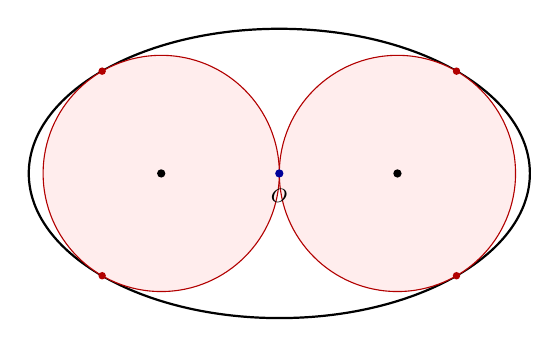
\begin{tikzpicture}[scale=1.5]
  \pgfmathsetmacro{\aa}{2.12132034}\pgfmathsetmacro{\bb}{1.22474487}\pgfmathsetmacro{\ty}{0.8660254}
  \draw[thick] (0,0) ellipse ({\aa} and {\bb});
  \draw[red!70!black,fill=red!7] (1,0) circle (1);
  \draw[red!70!black,fill=red!7] (-1,0) circle (1);
  \fill (1,0) circle (1.0pt); \fill (-1,0) circle (1.0pt); \fill[blue!60!black] (0,0) circle (1.0pt);
  \foreach \sx in {1,-1}{\foreach \sy in {1,-1}{\fill[red!70!black] (\sx*1.5,\sy*\ty) circle (0.9pt);}}
  \node[below] at (0,-0.05) {\scriptsize $O$};
\end{tikzpicture}
\end{center}

This value was found \emph{numerically} by James Buddenhagen in 2004 and listed on Erich Friedman's
Packing Center, but it had \textbf{never been proved}. The work described here is a complete proof,
\textbf{formally verified by the Lean~4 proof assistant} (with mathlib): the machine has checked every
inference down to the axioms of mathematics.

\section{Why this needs a proof at all}

It is tempting to think the answer is ``obvious'' once you see the picture --- but a picture is not a
proof, and here the difficulty is real:

\begin{itemize}
\item \textbf{It is an optimisation over infinitely many shapes.} An ellipse has five degrees of
freedom (two axis lengths, a centre, a tilt angle), and the two circles can sit anywhere disjoint
inside it. ``Smallest'' means smaller than \emph{every} other valid configuration --- an infinite
search. Showing a \emph{lower bound} (nothing can do better than $\tfrac{3\sqrt3}{2}\pi$) is the hard
half; the pretty picture only gives the \emph{upper} bound (this particular ellipse works).

\item \textbf{No elementary bound is tight.} Crude estimates (total area of the two circles, or the
width needed) only give $A \ge 2\pi$ and similar --- far below the true $8.16$. The exact value is
forced by a subtle interaction between the ellipse's eccentricity and where the circles can touch; it
does not fall out of any one-line inequality.

\item \textbf{Numerical evidence is not proof.} ``I ran an optimiser and it always returned
$8.1621$'' is strong evidence the value is right, but it is exactly what a numerical guess is --- it
cannot rule out a slightly better configuration the optimiser never tried, and it says nothing about
\emph{why}. That gap --- between ``the computer keeps finding this'' and ``this is provably optimal''
--- is what a proof closes, and what stood open from 2004 until now.
\end{itemize}

\section{The Lean statement (the thing the machine verified)}

The central theorem, verbatim from the Lean development:

\begin{lstlisting}[style=lean]
theorem area_toReal_ge_of_feasibleGen (A B C : Real) (c : Real x Real)
    (hfeas : FeasibleGen A B C c) :
    3 * Real.sqrt 3 / 2 * Real.pi <= (MeasureTheory.volume (ellipseGenSet A B C c)).toReal
\end{lstlisting}

\noindent In words: \emph{for every ellipse (described by $A,B,C,c$) that contains two
interior-disjoint unit circles, its area is at least $\tfrac{3\sqrt3}{2}\pi$.} Together with a second
theorem showing the optimal ellipse \emph{achieves} this value, that pins the minimum exactly.

Everything in the statement is built from standard, plain definitions --- this matters, because the
proof assistant guarantees ``the proof matches \emph{this} statement,'' so a human only needs to be
convinced \emph{the statement says what we mean}:

\begin{lstlisting}[style=lean]
-- A general (possibly tilted, off-centre) ellipse  (x-c)^T M (x-c) <= 1,  M = [[A,B],[B,C]]:
def ellipseGenSet (A B C : Real) (c : Real x Real) : Set (Real x Real) :=
  { x | A*(x.1-c.1)^2 + 2*B*(x.1-c.1)*(x.2-c.2) + C*(x.2-c.2)^2 <= 1 }

-- A genuine closed unit disk (Euclidean):
def diskSet (cx cy : Real) : Set (Real x Real) := { p | (p.1-cx)^2 + (p.2-cy)^2 <= 1 }

-- "The ellipse is a genuine ellipse and holds two interior-disjoint unit disks":
def FeasibleGen (A B C : Real) (c : Real x Real) : Prop :=
  0 < A  and  0 < A*C - B^2  and          -- positive-definite (Sylvester) => a real ellipse
  exists d1 d2,  diskSet d1 ⊆ ellipseGenSet A B C c
              and diskSet d2 ⊆ ellipseGenSet A B C c
              and 4 <= (d1-d2).normSq        -- centres >= 2 apart  =  disjoint interiors
\end{lstlisting}

\noindent The condition $0<A$ and $0<AC-B^2$ is exactly the test that the matrix
$M=\bigl(\begin{smallmatrix}A&B\\B&C\end{smallmatrix}\bigr)$ is positive definite, i.e.\ that the set
really is an ellipse (not a parabola or hyperbola); the area is then $\pi/\sqrt{\det M}$. The disks are
genuine Euclidean unit disks, ``$\subseteq$'' is genuine set containment, and ``centres $\ge 2$ apart''
is proved (in a companion lemma \texttt{interior\_disjoint\_iff}) to be \emph{equivalent} to the disks'
interiors being disjoint. The area is the genuine Lebesgue measure \texttt{MeasureTheory.volume}.

\section{What ``formally verified'' buys you here}

The proof was checked by Lean's small, trusted kernel. Running
\begin{lstlisting}[style=lean]
#print axioms area_toReal_ge_of_feasibleGen
  -- => [propext, Classical.choice, Quot.sound]
\end{lstlisting}
reports that the theorem rests on \emph{only} the three standard axioms of mathlib and \textbf{no
\texttt{sorry}} (no unproven step) --- transitively, through every lemma it depends on. There is no
room for a hand-wave, a missed case, or a ``looks true'' that is subtly false: the machine would have
rejected it. (This matters: an earlier, harder packing problem we attempted produced several
confident-looking but \emph{wrong} lemmas that only an external check caught. Here the kernel enforces
honesty mechanically.)

The proof also covers the \emph{fully general} ellipse --- arbitrary tilt $B\neq0$ and arbitrary
centre $c$ --- via a kernel-checked rigid-motion reduction (the tilt is rotated away by an explicitly
constructed eigenvector; rotations and translations preserve area and the disks). So nothing is
assumed about the ellipse being axis-aligned.

\section{What a reader still has to take on trust}

Honestly stated: the kernel proves \emph{the proof matches the statement above}. It does \emph{not}
know that the statement is the ``right'' question --- that is the one judgement a human must make, by
reading the five definitions in \S3 and agreeing they faithfully encode ``two unit circles, disjoint
interiors, smallest-area ellipse, real area.'' Those definitions are deliberately plain and built from
mathlib primitives precisely so that this final human check is short. Beyond that, the trust reduces to
trusting Lean's kernel and mathlib --- the same basis as any modern formalised theorem (Four Colour,
Kepler, etc.).

\vfill
\noindent\footnotesize Companion files: \texttt{lean/} (the Lean development, builds clean),
\texttt{AUDIT\_THIS.md} (the step-by-step audit checklist), and
\texttt{proof\_ellipse\_n2.tex} (the human-readable hand proof the formalisation follows).
\end{document}
